\documentclass{lug}

\title{OpenGL \& Computer Graphics}
\author{Sam Sartor}
\institute{Mines Linux Users Group}

\usepackage{etoolbox}
\usepackage{array}
\usepackage{amsmath}
\usepackage{adjustbox}

\makeatletter
\patchcmd{\beamer@sectionintoc}{\vskip1.5em}{\vskip0.5em}{}{}
\makeatother

\begin{document}

\newcommand{\pmidg}[1]{\parbox{\widthof{#1}}{#1}}

\begin{frame}{What is Computer Graphics?}
\begin{center}
    \pmidg{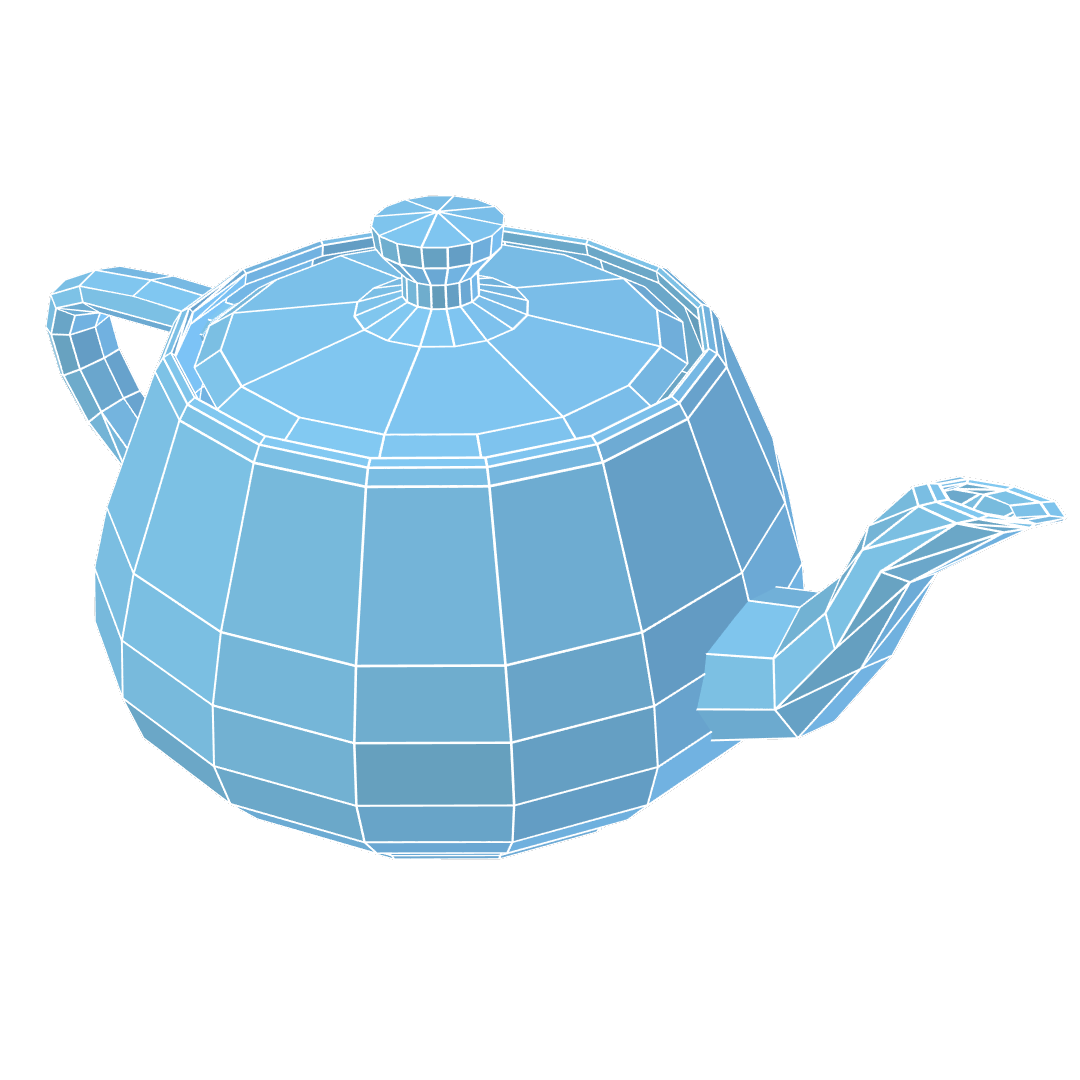
\includegraphics[width=4cm]{graphics/teapot_mesh}} \scalebox{2}{$\rightarrow$} \pmidg{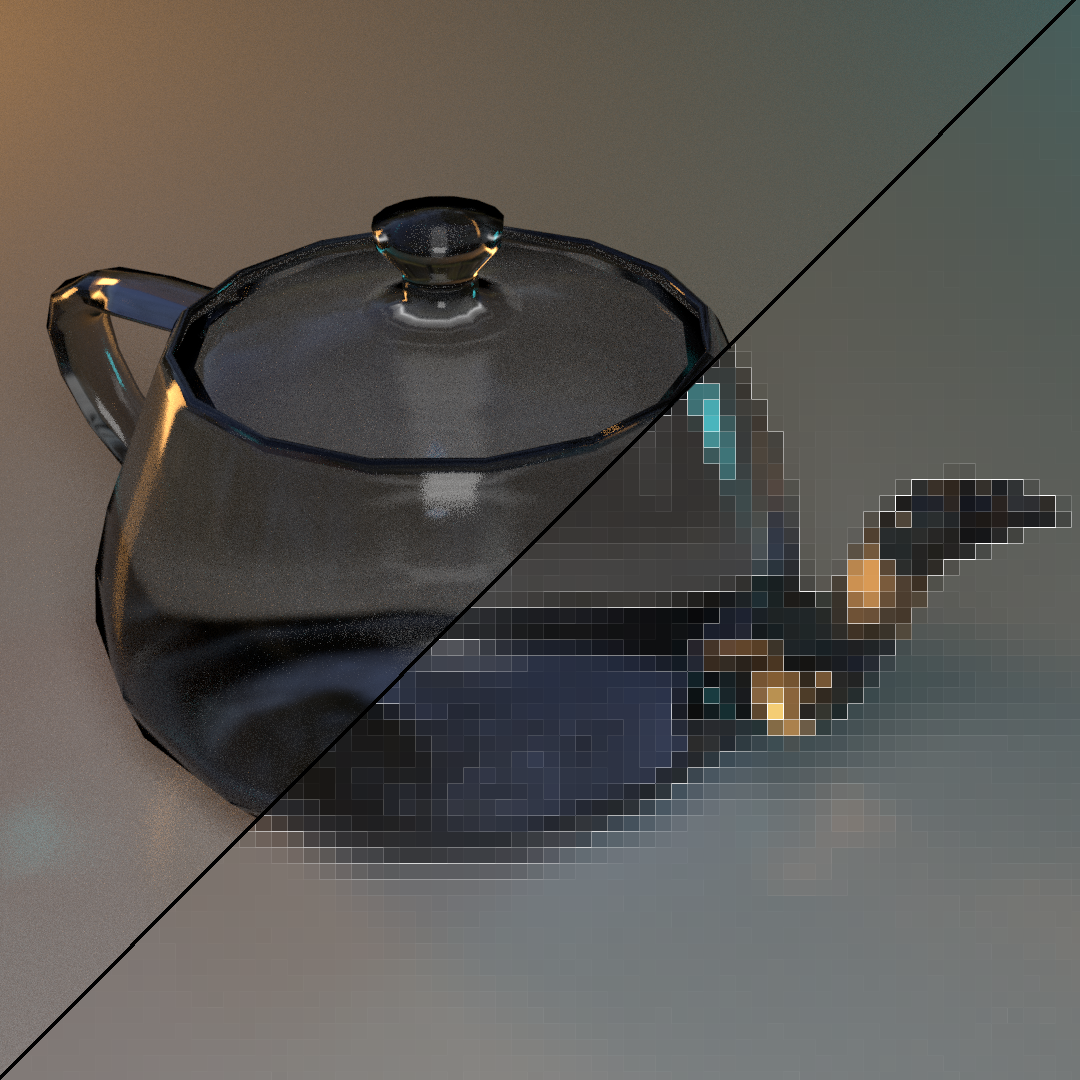
\includegraphics[width=4cm]{graphics/teapot_rt_pix}} \\
    
    \bigskip

    Computer graphics is the science of turning \textit{shapes} into \textit{pixels}.
\end{center}
\end{frame}

\begin{frame}{What is Computer Graphics?}
    \noindent
    \begin{minipage}{.65\textwidth}
        Computer Graphics is everywhere!
        \begin{itemize}
            \item Your terminal \\
            \item Web browsers \\
            \item Video games \\
            \item CAD software \\
            \item Movies, TV Shows \\
            \item The Ikea Catalog \\
            \item Your bootloader \\
            \item QT, GTK+, wxWidgets \\
            \item Vim, Emacs, Notepad \\
            \item Embedded devices \\
        \end{itemize}
    \end{minipage}% This must go next to `\end{minipage}`
    \begin{minipage}{.35\textwidth}
        \pmidg{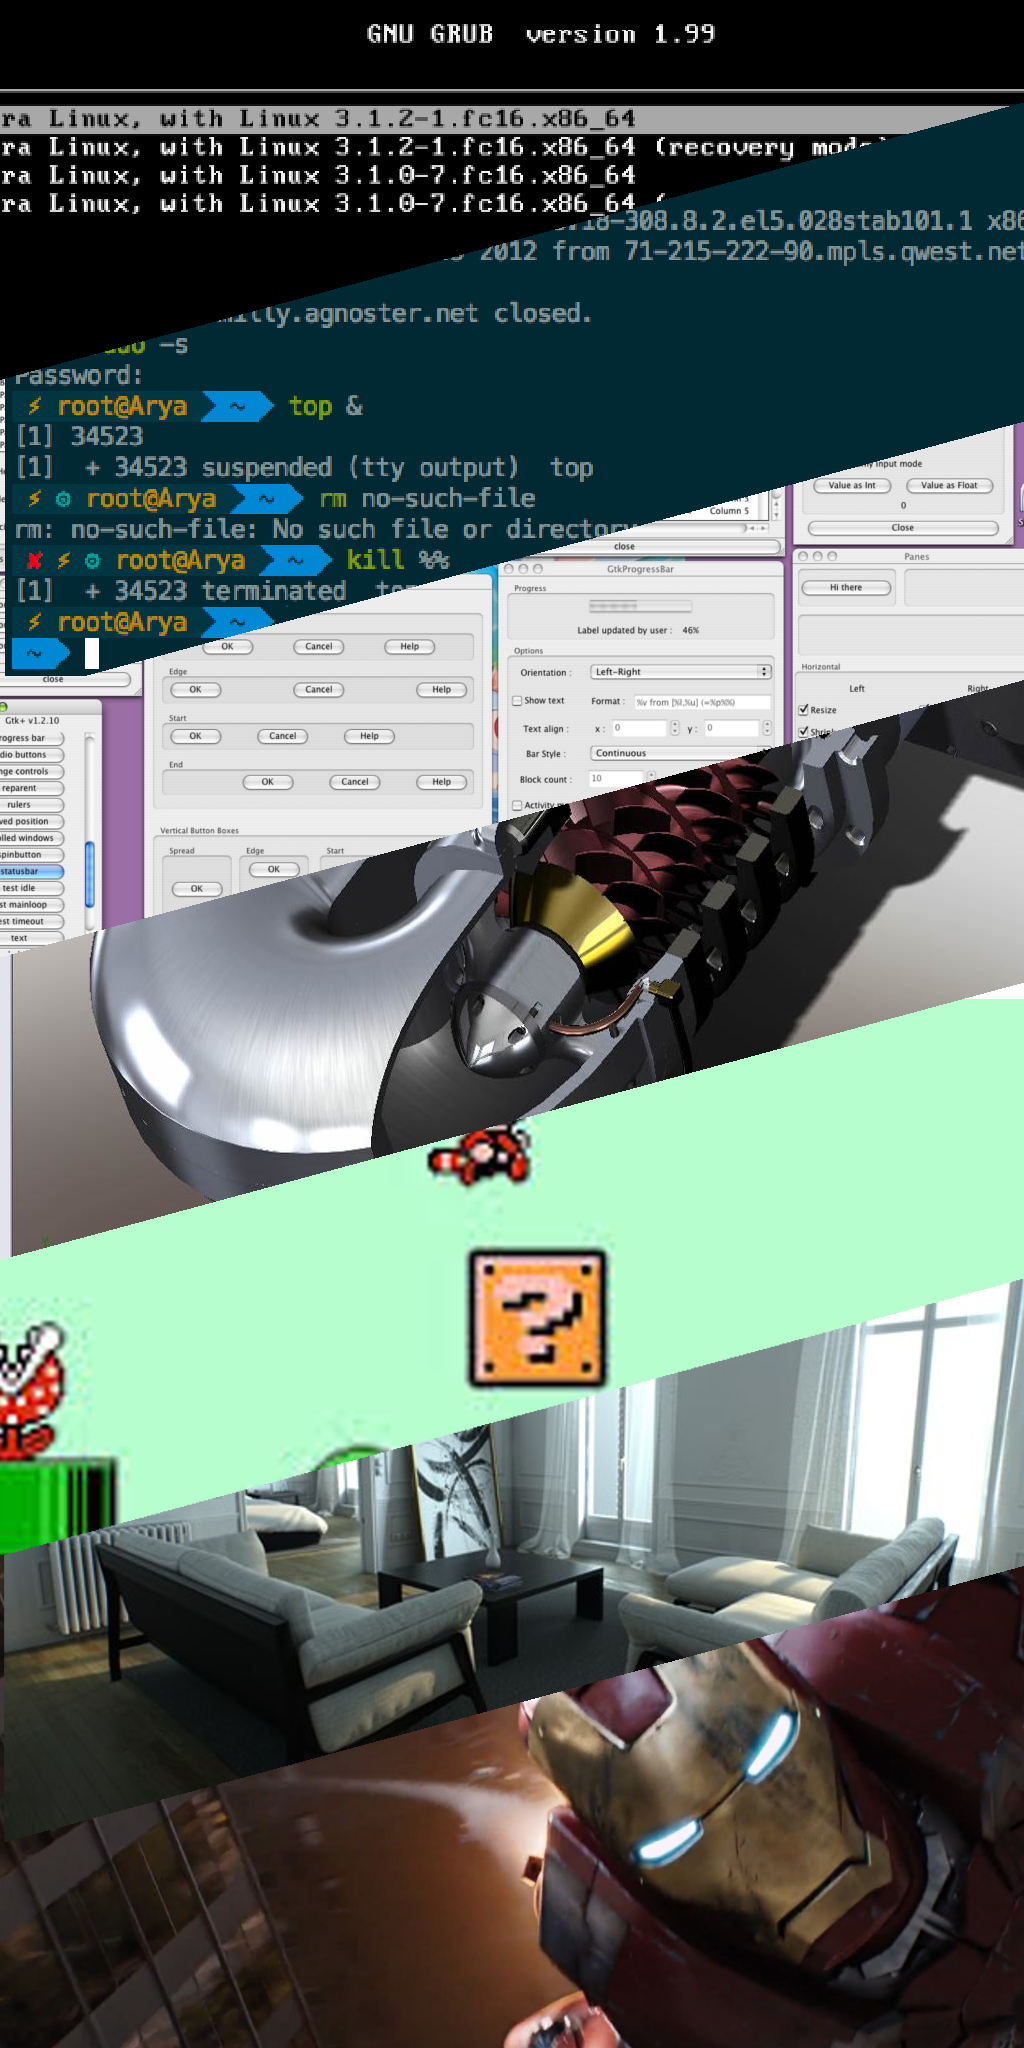
\includegraphics[width=\textwidth]{graphics/uses}}
    \end{minipage}
\end{frame}

\begin{frame}{Offline vs Online}
\end{frame}

\begin{frame}{History}
\end{frame}

\end{document}
